\documentclass[12pt]{article}

\usepackage[utf8]{inputenc}
\usepackage{latexsym,amsfonts,amssymb,amsthm,amsmath}
\usepackage{float}

\setlength{\parindent}{0in}
\setlength{\oddsidemargin}{0in}
\setlength{\textwidth}{6.5in}
\setlength{\textheight}{8.8in}
\setlength{\topmargin}{0in}
\setlength{\headheight}{18pt}
\usepackage{graphicx}

\usepackage{hyperref}
\hypersetup{
    colorlinks=true,
    linkcolor=blue,
    filecolor=magenta,      
    urlcolor=cyan,
    pdftitle={Overleaf Example},
    pdfpagemode=FullScreen,
    }

\urlstyle{same}

\usepackage{caption}
\DeclareCaptionFormat{citation}{%
  \ifx\captioncitation\relax\relax\else
    \captioncitation\par
  \fi
  #1#2#3\par}
\newcommand*\setcaptioncitation[1]{\def\captioncitation{\textit{Source:}~#1}}
\let\captioncitation\relax
\captionsetup{format=citation,justification=centering}


\title{MATH1034OL1 Pre-Calculus Mathematics Notes from Final Exam Review (Wednesday)}
\author{Elijah Renner}

\begin{document}

\maketitle

\vspace{0.5in}

\tableofcontents

\section{Notes During Final Exam Review}

The previous class notes I've written contain all topics that should be reviewed for the midterm. I haven't been taking notes for the midterm review. Instead, I've been referencing the previous notes to review. Here I'll just record any new information that's discussed in class.\\

Please find all lecture notes and their summaries here: \url{https://tamath.org/precalculus.html}.\\

On Friday, I'll post a large document containing all of the material from the course! I'll also add mini documents with any new mini details covered.\\


%%%%% FIGURE: %%%%%
%
%\begin{figure}[H]
%	\centering
%	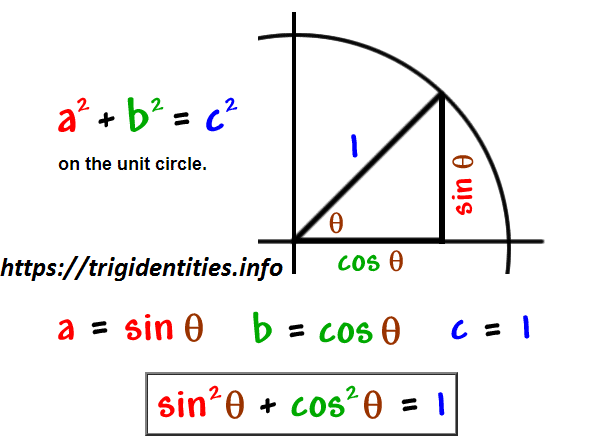
\includegraphics[scale=0.4]{Pythagorean Identity.png}
%	\caption{Credit: \url{https://trigidentities.info/pythagorean-trig-identities}}
%\end{figure}

\end{document}
